\documentclass[]{article}
\usepackage{amsmath}
\usepackage{amsfonts}
\usepackage[T1]{fontenc}
\usepackage[utf8]{inputenc}
\usepackage{graphicx}
\usepackage{xcolor}
\usepackage{pgfplots}
\pgfplotsset{width=5.5cm,compat=1.9}
\usepackage{titling}
\usepackage{multicol}
\newcommand{\HRule}{\rule{\linewidth}{0.5mm}} %linha horizontal
\begin{document}

\begin{titlingpage}
  \begin{center}

    \vspace*{1cm}
    \textsc{\large Technische Universität München}\\[1.5cm]
    \textsc{\Large Math 3}\\[0.5cm]
    \textsc{\large MA9803 | B.Sc. Engineering Science and B.Sc. Aerospace}\\[0.5cm]

    \HRule\\[0.4cm]
    {\huge\bfseries Modeling and Simulation with Ordinary Differential Equations}\\[0.4cm]
    \HRule\\[0.4cm]

    \begin{minipage}{0.4\textwidth}
      \begin{flushleft}
        \scriptsize
        \;\,\textit{Lecturer}\\[1ex]
        \begin{tabular}{ll}
           Prof. Dr. Elisabeth Ullmann &\\
        \end{tabular}
      \end{flushleft}
    \end{minipage}
    ~
    \begin{minipage}{0.4\textwidth}
      \begin{flushright}
        \small
        \textit{Notes by}\\
	Rangi Siebert\\

      \end{flushright}
    \end{minipage}

    \vfill\vfill\vfill

    {\large\today}

    \vfill
  \end{center}

\end{titlingpage}

\begin{abstract}
	Some people think that stiff challenges are the best device to induce learning, but I am not one of them. The natural way to learn something is by spending vast amounts of easy, enjoyable time at it. This goes whether you want to speak German, sight-read at the piano, type, or do mathematics. Give me the German storybook for fifth graders that I feel like reading in bed, not Goethe and a dictionary. The latter will bring rapid progress at first, then exhaustion and failure to resolve. 
	\par\small \textit{L. N. Trefethen. Trefethen’s index cards - Forty years of notes about People, Words and Mathematics. World Scientific, 2011, S. 86}
\end{abstract}
\tableofcontents
\newpage


\section{Introduction}
	\paragraph{Previously:}
	We had equations like  $y ^{2}+4y+1=0$, where the solution is a number.
	\[
		\int_{a}^{b} f(x) dt = \text{number} = F(b)-F(a)	
	\]
	\paragraph{New:}
	$ f'(x) $ is given, determine $ f(x) $. The solution is a function.
	\[
		\begin{split}
			\text{Velocity}(t) & = \text{Position}'(t)~~~~  \text{given}  \\
					   & = \text{Position}(t)~~~~~  \text{wanted}
		\end{split}
	.\]
	\subsection{Differential Equations}
	\begin{multicols}{2}
	\paragraph{Example:
	Interest rate}
	$~$\\
	$y(t):~~$ assets at time $t$. \\
	$\lambda<0:$ constant interest rate.
	\[
	\begin{split}
		\text{IVP}&
	\begin{cases} 
		y'(t) & =\lambda\cdot y(t), \\
		y(0) & =y_0.
	\end{cases}\\
	\end{split}
	\]$~$
	\begin{center}
	\begin{tikzpicture}
	\begin{axis}[
		axis lines = left,
		xlabel = \(t\),
		ylabel = {\(y\)},
		ymin=1,
		ymax=4,
		xmax=1,
		xtick={9},
		ytick={2},
		yticklabels={$y_0$},
		x label style={at={(axis description cs:1,-0.05)},anchor=north},
    		y label style={at={(axis description cs:-0.05,1)},rotate=-90,anchor=east},
	]
	%Below the red parabola is defined
	\addplot [
		domain=0:2, 
		samples=100, 
		color=blue,
		]
		{x^2+2};
	\addlegendentry{\(y=y(t)\)}
		\end{axis}
	\end{tikzpicture}
	\end{center}	
	\end{multicols}
	\paragraph{Example: Radioactive Decay}
	$~$\\$y(t):~~~$ mass of a substance at time $t$.\\
	$\lambda<0:$ decay rate.
	\[
	\begin{split}
	y'(t)=  \lambda &\cdot y(t)
	\end{split} 
	.\]
\subsection{Problem Solving Steps in Science \& Technology}
	"Reality" $ \longrightarrow $ Model = "Mathematisation"
	\begin{itemize}
		\item Laws of nature (Physics, Chemistry).
		\item Assumtions, hypoteses $ \rightarrow $ differential equations.
		\item Analytical or symbolic solution (exact solution). \textcolor{red}{not practical} 
		\item Numerical solution. \textcolor{teal}{in practise}
	\end{itemize}
	\[
		\text{ \textbf{Change of state}  }= \text{ \textbf{Function (State)}}
	.\]
	\paragraph{Ordenary Diff. Eqn. (ODE:} one scalar variable (e.g. time) \textcolor{red}{this semester}
	\[
	y'(t)=\lambda y(t)
	.\]
	\paragraph{Partial Diff. Eqn. (PDE):} multiple variables (e.g. time and space) \textcolor{teal}{next semester (MA9804)}
	\[
		u=u(t,x)\,\,\,~~x=(x_1,x_2,x_3) 
	.\]
	\[
		\frac{\delta u}{\delta t}=k \cdot \big( \frac{\delta ^{2}u}{\delta x_1 ^{2}}\frac{\delta ^{2}u}{\delta x_2 ^{2}}\frac{\delta ^{2}u}{\delta x_3 ^{2}}\big)
	.\]
	\begin{center}
		\textcolor{darkgray}{Heat equation. $u$: temperature}
	\end{center}

	\paragraph{Oftentimes:} Solution depends on (design) parameters. $y=y(t;\rho)$, $u=u(t,x,\rho)$
	\begin{itemize}
		\item Parameter identification \textcolor{teal}{Inverse Problem}
		\item Design optimisation
		\item Random / Stochastic parameters \textcolor{blue}{Uncertainty quantification}
	\end{itemize}
	\subsection{Application: Solid Mechanics}
	\paragraph{Newton's Laws of motion:} $ \frac{dp}{dt}=F $ 
	\[
	\text{Change of momentum}= \text{force action}
	.\]
	\begin{enumerate}
		\renewcommand{\labelenumi}{\alph{enumi})}
		\item Calculate orbits of satellites; today: GPS
		\item Vibrations in automobiles; reliability of structures. (earthquakes; spring-mass-system)
	\end{enumerate}
	
	\subsection{Application: Electric Ciruits}
	\paragraph{Ohm's Law:} $ U=R \cdot I $ (voltage = resistance * current)
	\paragraph{Kirchhoff's Cirquit Laws:} $\rightarrow$ System of ODEs
	\paragraph{Law of Induction:} $ U=n \cdot I' $ (Coil); $ I = C \cdot U' $ (Capacitor). Here the $'$ is the time derivative.
	\subsection{Application: Chemical relations}
	\paragraph{Chemical reaction:} $ A+B\underset{k}\longrightarrow C $. \\  Here $c_A(t), c_B(t), c_C(t)$ are the Concentrations of the substance $A,B,C$ in $ \frac{ \text{Mol}}{\text{l}}$. 
	\paragraph{Law of mass action:} 
	Change of concentration is proportional to the concentration of the resulting substances:
	\[
	\begin{split}
		 & c_C'=~k \cdot c_A \cdot c_B \\
		 & c_A'=-k \cdot c_A \cdot c_B \\
		 & c_B'=-k \cdot c_A \cdot c_B \\
	\end{split}
	\]
	\subsection{Classification of ODEs}
	\[
	y(x)
	.\]
	\begin{multicols}{2}
	$x$: independent variable \textcolor{teal}{scalar}\\
	$y$: dependent variable
	\end{multicols}
	\paragraph{Ordenary DE:}
	\begin{itemize}
		\item System of ODEs:
			$
			y(x)\in\mathbb R ^{n},n>1
			.$
		\item Single ODE:
			$ ~~~~~~~
			y(x) \in\mathbb R,n=1
			.$
	\end{itemize}
	\paragraph{Implicit DE of order $m$:} 
	\[
	F\big(x,y(x),y'(x),...,y ^{(m)}(x)\big) = 0
	.\]
	\paragraph{Explicit DE of order $m$:}  
	\[
	y ^{(m)}(x)=f\big(x,y(x),y'(x),...,y ^{(m-1)}(x)\big)
	.\]
	
\section{First-order ODEs}
For now we have $ m=1,n=1 $. Consider $y'(x)=f\big(x,y(x)\big)$. The \textbf{explicit form} of the ODE is noted like $ y'=f(x,y) $ explicit form of ODE. The function $ f $ is defined on $D=D_x\times D_y\in\mathbb R ^{2}$.
\subsection{Examples}
\paragraph{"Strip":}
\begin{multicols}{2}
\begin{center}
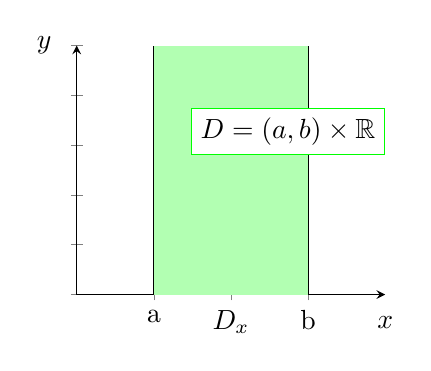
\begin{tikzpicture}
	\begin{axis}[
		axis lines = left,
		xlabel = \(x\),
		ylabel = {\(y\)},
		xmin=-10, xmax=10,
		ymin=0, ymax=10,
		xtick={-5, 5,0}, xticklabels={a,b,$D_x$},
		ytick={}, yticklabels={},
		x label style={at={(axis description cs:1,-0.05)},anchor=north},
    		y label style={at={(axis description cs:-0.05,1)},rotate=-90,anchor=east},
	]
	\addplot[black, thick] coordinates {(-5, 0) (-5, 10)};
	\addplot[black, thick] coordinates {(5, 0) (5, 10)};
	\addplot[fill=green!30, draw=none] coordinates {(-5, 0) (5, 0) (5, 10) (-5, 10)};
	\node[anchor=north east, draw=green, fill=white] at (200,75) {$D= (a,b)\times \mathbb R$};
		\end{axis}
	\end{tikzpicture}
\end{center}
	\begin{center}
	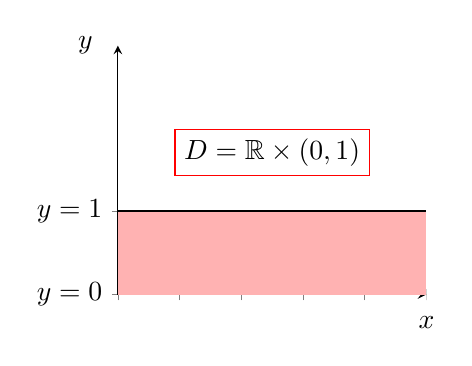
\begin{tikzpicture}
		\begin{axis}[
			axis lines = left,
			xlabel = \(x\),
			ylabel = {\(y\)},
			xmin=0, xmax=10,
			ymin=0, ymax=3,
			xtick={}, xticklabels={},
			ytick={0,1}, yticklabels={$y=0$,$y=1$},
			x label style={at={(axis description cs:1,-0.05)},anchor=north},
	    		y label style={at={(axis description cs:-0.05,1)},rotate=-90,anchor=east},
		]
			\addplot[black, thick] coordinates {(0, 1) (10, 1)};
			\addplot[fill=red!30, draw=none] coordinates {(0,0) (0, 1) (10, 1) (10, 0)};
			\node[anchor=north, draw=red] at (50,200) {$D= \mathbb R\times (0,1)$};
		\end{axis}
		\end{tikzpicture}
	\end{center}
\end{multicols}
	\paragraph{"Rectangle":} 	
	\begin{center}
	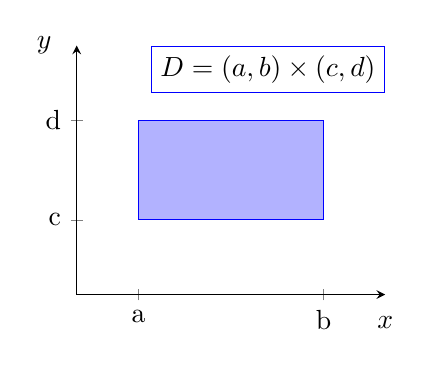
\begin{tikzpicture}
		\begin{axis}[
			axis lines = left,
			xlabel = \(x\),
			ylabel = {\(y\)},
			xmin=0, xmax=10,
			ymin=0, ymax=10,
			xtick={2,8}, xticklabels={a,b},
			ytick={3,7}, yticklabels={c,d},
			x label style={at={(axis description cs:1,-0.05)},anchor=north},
	    		y label style={at={(axis description cs:-0.05,1)},rotate=-90,anchor=east},
		]
			\addplot[fill=blue!30, draw=blue, mark=none] coordinates {(2,3) (8, 3) (8, 7) (2, 7) (2,3)};
			\node[anchor=north east, draw=blue] at (100,100) {$D=(a,b)\times(c,d)$};
		\end{axis}
	\end{tikzpicture}
	\end{center}
	
\subsection{Geometric Interpretation: Direction Field}
\begin{multicols}{2}
\begin{center}
\begin{tikzpicture}
	\begin{axis}[
		axis lines = left,
		xlabel = \(x\),
		ylabel = {\(y\)},
		xmin=0, xmax=1,
		ymin=0, ymax=2,
		xtick={11}, xticklabels={11},
		ytick={11}, yticklabels={11},
		x label style={at={(axis description cs:1,-0.05)},anchor=north},
    		y label style={at={(axis description cs:-0.05,1)},rotate=-90,anchor=east},
	]
		\addplot [
			domain=.1:1.8,
			samples=100,
			color=black,
			]
			{((x)^2+1};
		\fill[red] (50, 125) circle (3pt);
		\addplot[black, thin, gray] coordinates {(.25, 1) (.75, 1.5)};
		\fill[red] (50, 75) circle (3pt);
		\addplot[black, thin, gray] coordinates {(.25, .5) (.75, 1)};
	\end{axis}
\end{tikzpicture}
\end{center}
$~$
\[
y'=f(x,y)
.\]
$f(x,y)$: Slop of tangent line of $y(x)$ in point $(x,y)$. Using software like \textit{dfield} we can visualize $f(x,y)$ as an vector field.
\end{multicols}
\subsection{Observations}
\begin{enumerate}
	\item Through each point $ (x_0,y_0)\in D $ there passes \textbf{exactly one} solution curve.
	\item Each solution curve is \textbf{maximal}, meaning that the curve continues until the boundary of $D$ (this includes a blow up to $+\infty$).
	\item Solution curves \textbf{don't intersect}!
		\begin{multicols}{2}
		\begin{center}
		\begin{tikzpicture}
			\begin{axis}[
				axis lines = left,
				xlabel = \(x\),
				ylabel = {\(y\)},
				xmin=0, xmax=10,
				ymin=0, ymax=5,
				xtick={5}, xticklabels={ \textcolor{red}{$x_\infty$}},
				ytick={}, yticklabels={},
				x label style={at={(axis description cs:1,-0.05)},anchor=north},
		    		y label style={at={(axis description cs:-0.05,1)},rotate=-90,anchor=east},
			]
				\addplot[black, thick] coordinates {(3, 10) (3, 0)};
				\addplot[black, thick] coordinates {(7, 10) (7, 0)};
				\addplot [
					domain=3.3:4.9,
					samples=100,
					color=black,
					]
					{-1/(x-5)};
				\addplot[red, thin, dashed] coordinates {(5, -1) (5, 10)};
			\end{axis}
		\end{tikzpicture}
		\end{center}
		\begin{center}
		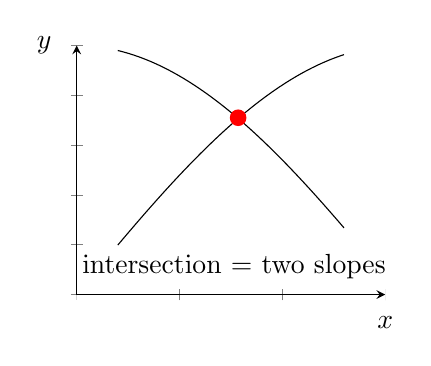
\begin{tikzpicture}
			\begin{axis}[
				axis lines = left,
				xlabel = \(x\),
				ylabel = {\(y\)},
				xmin=0, xmax=1.5,
				ymin=0, ymax=1,
				xtick={}, xticklabels={},
				ytick={}, yticklabels={},
				x label style={at={(axis description cs:1,-0.05)},anchor=north},
		    		y label style={at={(axis description cs:-0.05,1)},rotate=-90,anchor=east},
			]
			\addplot [
				domain=0.2:1.3,
				samples=100,
				color=black,
				]
				{cos(deg(x))};
			\addplot [
				domain=0.2:1.3,
				samples=100,
				color=black,
				]
				{sin(deg(x))};
				\fill[red] (78.5, 71) circle (3pt);
				\node[anchor=north east, draw=none] at (155,20) {intersection = two slopes};
			\end{axis}
		\end{tikzpicture}
		\end{center}
		\end{multicols}
	\end{enumerate}
	\subsection{Existence and Uniqueness of a Solution}
	IVP (initial value problem): $y'=f(x,y),$ $y(x_0)=y_0,$ domain $D$
	\subsubsection{Theorem:  Peano} Assume that $f$ is continuous on $D$ and $(x_0,y_0)\in D$. Then the IVP has at leas one solution. This solution is minimal, meaning that we can continue the solution for $x <x_0$ and $x > x_0$ until the boundary of $D$.
	\subsubsection{Theorem: Picard-Lindelöf} Let $f$ be continuous on $D$ and let $f$ be continuously differentiable with respect to $y$, that is, $ \frac{\delta f}{\delta y} $ is continuous. Let $(x_0,y_0)\in D$. Then the IVP has a unique solution.
	\paragraph{Example:}$~$ 
	\begin{multicols}{2}
	\begin{center}
	\textcolor{red}{implicit form of ODE}
	\end{center}
	\[
		(x ^{2}-x)y'=(2x-1)y,~~y(x_0)=y_0
	.\]
	\begin{center}
	\textcolor{teal}{explicit form}
	\end{center}
	\[
	y'= \frac{2x-1}{x ^{2}-x}y~~f(x,y)= \frac{2x-1}{x ^{2}-x}y
	.\]
	\end{multicols}
	\paragraph{Three cases:} 
	\begin{enumerate}
		\item $x_0\not\in \{0;1\}$: Unique solution (due to Picard-Lindelöf Thm.).
		\item $x_0\in \{0;1\}$ and $y_0=0$: Infinitely many solution\\$y(x)=cx(x-1),~c\in \mathbb R$ \textcolor{teal}{ Check it!}
		\item $x_0\in \{0;1\}$ and $y_0\not=0$: No solution.
	\end{enumerate}
\subsection{Examples and Recap}
\[
	\text{IVP}
	\begin{cases} 
		y' & =\lambda y, \\
		y(x_0) & =y_0.
	\end{cases}
\]
	$\lambda\in \mathbb R$ is a constant.
	\paragraph{a) Domain of Definition $D$}
	Here: \textcolor{teal}{$f(x,y)=\lambda y$} with $x$ being the independent and $y$ the dependent variable.
	\[
	D= \mathbb R\times \mathbb R
	.\]
	Meaning: $f$ is well defined for all $x\in \mathbb R$ and for all $y\in \mathbb R$
	\paragraph{b)} Direction field, software dfield, geometric interpretation.
	\paragraph{c)} Existence and uniquness of the soluton of the DE (differential equation).
	\paragraph{d)} $y(x)=c \cdot e ^{\lambda x},~~c\in \mathbb R$ is the g\underline{eneral solution} of the DE. Check:
	\[
	y'=c \cdot \lambda \cdot e ^{\lambda x}= \lambda c e ^{\lambda x}=\lambda y(x)
	.\]
	\textcolor{blue}{Parameter $c$ is determined by the initial condition}
	\[
	y(x_0)=ce ^{\lambda x_0 }\overset ! = y_0 \rightarrow c= y_0e ^{-\lambda x_0}
	.\]
	\paragraph{Remark on "general solution":} \textcolor{gray}{What does it mean?} Suppose the DE $y'=\lambda y $ has another solution $\overset \sim y$. Then it holds:
	\[
	\begin{split}
		\Bigg( \frac{\tilde y}{e ^{\lambda x}}\Bigg)'= & \frac{\tilde y' e ^{\lambda x}-\tilde y \lambda e ^{\lambda  x}}{(e ^{\lambda x}) ^{2}} \\
		= & \frac{e ^{\lambda x}(\tilde y'-\lambda \tilde y)}{e ^{2 \lambda x}}\\
		= & e ^{-\lambda x}\big(\tilde y'-\lambda \tilde y)=e ^{-\lambda x} \cdot 0 = 0 
	\end{split}
	\]
	\textcolor{gray}{$\tilde y'-\lambda \tilde y = 0$ since $\tilde y$ solves DE $\tilde y' = \lambda \tilde y$ by assumption.}\\
	Hence $ \dfrac{\tilde y}{e ^{\lambda x}}= \text{constant}$ and $\tilde y = \text{constant} \cdot e ^{\lambda x}$.\\
	Hence all solutions of $y'=\lambda y$ have the form $y=ce ^{\lambda x}$, $c\in \mathbb R$.
	\begin{multicols}{2}
	\paragraph{ \textcolor{red}{Today's topic}:} Analytical techniques for the solution of first-order differential equations.
	\paragraph{ \textcolor{blue}{Be careful}:} Techniques do not work for all DEs; require assumptions!
	\end{multicols}
	\subsection{Separation of Variables}
	\[
	y'(x) = f(x) \cdot g(y)
	.\]
	\begin{enumerate}
		\item Particular solution: The zeros of $g$ are stationary (constant) solutions.\\ \textbf{Example:} $g(y ^{*} = 0 \rightarrow \tilde y \equiv y ^{*}$ solves the DE. \\ \textbf{Check:} $0=(y ^{*})' = \tilde y' = f(x) \cdot g(y ^{*})$ \textcolor{gray}{$~~~~~~~g(y ^{*})=0$}
		\item If $f$ is continuous and $g$, $g'$ are continuous, we couclude with (2.4) that the DE has a unique solution (Picard-Lindelöf Theorem).
		\item Assume $g(y)\not=0$:
			\begin{enumerate}
				\item $\frac{dy}{dx}=f(x)g(x)$
				\item $ \frac{dy}{g(y)}= f(x) dx$ \textcolor{gray}{Separation of variables}
				\item $\int \frac{dy}{g(y)}= \int f(x) dx $ \textcolor{red}{$+c~~~$Parameter}
				\item Calculate the antiderivatives.
				\item If possible, rearrange (d). and isolate $y$.
			\end{enumerate}	
	\end{enumerate}	
	\subsection{Example, Separation of Variables}
	\[
	y'=-x ^{2}y~~~~~~~~~~~ \text{(see previous lecture)}
	.\]
	\begin{itemize}
		\item $f(x)=-x ^{2}$
		\item $g(y)=y$
	\end{itemize}
	\begin{enumerate}
		\item Stationary solution: $y\equiv 0$
		\item  
			\[
			\begin{split}
			\frac{dy}{dx} = & - x ^{2}y \\
			\frac{dy}{y} = & - x ^{2} dx \\
			\int \frac{dy}{y} = & - \int x ^{2} dx + c, \quad c \in \mathbb{R} \\
			\ln |y| = & -\frac{1}{3}x ^{3} + c \\
			|y| = & \exp\left( -\frac{1}{3} x ^{3} + c \right) = e ^{c} \cdot e ^{ - \frac{1}{3}x ^{3}}\quad \quad e ^{c} > 0 \\
			y = & \pm e ^{c} \cdot e ^{- \frac{1}{3}x ^{3}}\quad \text{plus}\quad y\equiv 0
			\end{split}
			\]
	\end{enumerate}
	\paragraph{Summary:}  $y(x)=\tilde c \cdot e ^{- \frac{1}{3}x ^{3}}$, $\quad\tilde c\in \mathbb R$ \begin{center}
	 \textcolor{blue}{general solution of DE}\\
	\end{center}
	From now on \textcolor{teal}{"antilogarithm"}: \[
	\begin{split}
		\ln|y| & = (...)+c,\quad c\in \mathbb R \\
		y & =\tilde c \cdot e ^{(...)},\quad \tilde c\in \mathbb R
	\end{split}
	\]
	\subsection{Application: Water Container}
	\paragraph{Given::} Cross-section area of cylindrical container $A$ and cross-section area of (circular) outlet $B$.
	\paragraph{Toricelli's Law:} 
	\[
		v_{out}=\sqrt {2gh}
	.\]
	\paragraph{Wanted:} $h=h(t)\quad$ water level in container.
	\paragraph{Question:} At which time is the container empty? For witch $t ^{*}$ does it hold $h(t ^{*})=0$?\\
	consider the change of volume $\Delta V$ of water in container.
	\[
	\begin{split}
		 \Delta V_{cont} &= A \cdot \Delta h \\
		 \Delta V_{out}& = \gamma \cdot B \cdot v_{out} \cdot \Delta t 
	\end{split}
	\]
	$\gamma$: Borda factor $\quad \gamma=0.62$ for circular outlet.
	\paragraph{Conservation of Mass:} 
	\[
		\begin{split}
			\Delta V_{cont}+\Delta V_{out} = &~ 0\quad\quad \Delta V_{cont}=-\Delta V_{out}  \\
			A \cdot \Delta h = & -\gamma \cdot B \cdot \sqrt{2gh}\Delta t\\
			A \cdot \frac{\Delta h}{\Delta t} = & -\gamma B\sqrt{2gh}\\
			\text{ \textcolor{gray}{$\Delta t\to 0$}}\quad\quad\quad\quad &\\
			A*h' = & -\gamma B\sqrt{2gh}\\
			\text{ \textcolor{red}{IVP} for }h(t) &
			\begin{cases} 
				 & h'(t)=-\gamma B\sqrt{2gh(t)} \\
				 & h(0)=h_0.
			\end{cases}
		\end{split}
	\]
	Solve my separation of variables!
	\begin{enumerate}
		\item $\tilde g(h) =\sqrt h$\\
			$\tilde f(t)=-\gamma \frac{B}{A}\sqrt{2g}$\\
			$h'(t)=\tilde f(t) \cdot \tilde g(h)$\\
			Stationary solution: $h\equiv 0$ is zero of $\tilde g(h) = \sqrt h$.
		\item Domain of definition: $D= \mathbb R\times [0,\infty)$ \textcolor{gray}{(time $t$ $\times$ water level $h$)}
			\begin{multicols}{2}
			\begin{center}
			\begin{tikzpicture}
				\begin{axis}[
					axis lines = left,
					xlabel = \(h\),
					ylabel = {\( \)},
					xmin=0, xmax=10,
					ymin=0, ymax=5,
					xtick={0}, xticklabels={$h=0$},
					ytick={0}, yticklabels={},
					x label style={at={(axis description cs:1,-0.05)},anchor=north},
			    		y label style={at={(axis description cs:-0.05,1)},rotate=-90,anchor=east},
				]
					\addplot [
						domain=0:10,
						samples=100,
						color=blue,
						]
						{sqrt(x)};
					\addlegendentry{\(\sqrt h\)}
				\end{axis}
			\end{tikzpicture}
			\end{center}
			$\quad$
			\[
				\begin{split}
					h\ge 0 \quad & \text{existence (Peano)} \\
				h >0\quad & \text{existence and uniqueness}\\
					  & \text{(Picard-Lindelöt)}
				\end{split}
			.\]
			\end{multicols}
		\item Separation of variables.
		\[
		\begin{split}
		\text{let } \mu & := \gamma \frac{B}{A}\sqrt{2g},\quad h > 0 \\
		\frac{dh}{dt} & = -\mu \sqrt{h} \\
		\int \frac{dh}{\sqrt{h}} & = -\mu \cdot \int 1 \cdot dt + c \\
		2\sqrt{h} & = -\mu \cdot t + c
		\end{split}
		\]
	\end{enumerate}	
	\paragraph{Initial condition:} $h(0)= h_0 > 0 \rightarrow c=\sqrt h_0$ \textcolor{gray}{$=-\mu \cdot 0+c$}\\
	$2\sqrt h = -\mu \cdot t + 2\sqrt h_0\quad$ \textcolor{gray}{Rearrange, isolate $h$}\\
	$h(t)= \frac{1}{4}(2\sqrt h_0 - \mu t ) ^{2}\quad$ \textcolor{orange}{as long as $h >0$!}
	\begin{multicols}{2}
	\begin{center}
	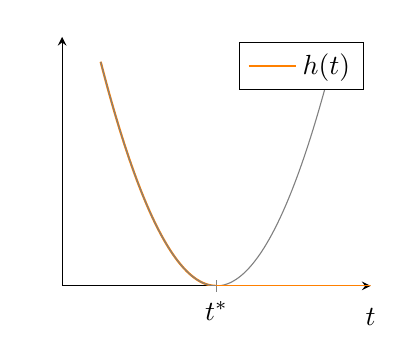
\begin{tikzpicture}
		\begin{axis}[
			axis lines = left,
			xlabel = \(t\),
			ylabel = {\( \)},
			xmin=-4, xmax=4,
			ymin=0, ymax=10,
			xtick={0}, xticklabels={$t ^{*}$},
			ytick={0}, yticklabels={},
			x label style={at={(axis description cs:1,-0.05)},anchor=north},
	    		y label style={at={(axis description cs:-0.05,1)},rotate=-90,anchor=east},
		]
			\addplot [
				domain=-3:0,
				samples=100,
				color=orange,thick
				]
				{x*x};
			\addplot [
				domain=-3:3,
				samples=100,
				color=gray,thin
				]
				{x^2};
			\addlegendentry{\(h(t)\)}
			\addplot[orange,thick] coordinates {(0, 0) (4, 0)};
		\end{axis}
	\end{tikzpicture}
	\end{center}
	\paragraph{Complete Solution:} 
	\[
	h(t) =
	\begin{cases} 
	\frac{1}{4}(2\sqrt h_0-\mu t) ^{2}\quad & t\le t ^{*}, \\
		0 & t >t ^{*}.
	\end{cases}
	\]
	\[
	\begin{split}
		\text{When is }h(t ^{*}) & =~0\\
		2\sqrt h_0 & =~\mu t ^{*}\\
		t ^{*} & = ~ \frac{2\sqrt h_0}{\mu}.
	\end{split}
	\]
	\end{multicols}

	\subsection{Linear DE of first Order}
	\paragraph{Standard form:} $ y'(x)=+p(x)y(x)=r(x) \quad$ \textcolor{blue}{$p,r$ can be nonlinear functions in $x$}\\
	DE is linear in $y,y'$, not allowed are terms like $(y') ^{2},\sin(y),y \cdot y'$ etc.
	\[
		\begin{split}
			p=p(x),r=r(x) \text{ continuous} \rightarrow & \text{ existance and uniqueness}  \\
			 & \text{solution}
		\end{split}
	.\]
		\paragraph{Recall:} $y'=f(x,y)$
		\paragraph{Here:} \[
		\begin{split}
			y'= &~ r(x)-p(x) \cdot y(x) \text{ \textcolor{blue}{$=:f(x,y)$}} \\
			\frac{\delta f}{\delta y} = & -p(x)
		\end{split}
		.\]
		\paragraph{Concepts:} 
		\[
		\begin{split}
			y'(x)+p(x)y(x) = 0\quad & \text{homogeneous linear DE} \\
			y*(x)+p(x)y(x)=r(x)\quad & \text{inhoogenous linear DE }r(x)\not\equiv0
		\end{split}
		\]
		\paragraph{ \underline{Remarks}:}
		\[
			\begin{split}
				Ax = b \quad & \text{linear system of equations} \\
				Ax=0\quad & \text{homogeneous linear system of equations} \\
				b\not=0\quad & \text{inhomogeneous linear system of equations.}
			\end{split}
		\]
		\subsection{General Solution of the homogeneous DE}
		\[
		\begin{split}
			y*(x) + p(x)y(x)= & ~0\quad\quad y'= \frac{dy}{dx}  \\
			\frac{dy}{dx}= &-p(x)y(x) 
		\end{split}
		\]
		Variables of $p(x)$ and $y(x)$ are separate.
		\begin{enumerate}
			\item Stationary solution: $y\equiv 0$
			\item $y\not=0$, separation of variables.
				\[
				\begin{split}
				\frac{dy}{dx} & =-p(x)y(x) \\
				\int \frac{dy}{y} &= - \int_{x_0}^{x} p(z) dz+c\\
				ln|y| &=- \int_{x_0}^{x} p(z) dz+c \text{ \textcolor{blue}{$=P(x)-P(x_0)+c$}}\\
				      &=-P(x)+\tilde c
				\end{split}
				\]
				\textcolor{blue}{Let $P( \cdot )$ denote the antiderivative of $p( \cdot )$}, that is, $P
				(z)=p(z)$.
		\end{enumerate}
		\paragraph{ \textcolor{teal}{"antilogarithm":}} \[
			y(x)=\hat c \cdot e ^{-P(x)},\quad \hat c\in \mathbb R
		.\]
		\paragraph{ \underline{Reminder}:} $ \int_{x_0}^{x} p(z)dz =: F(x)$
		\[
		\frac{dF}{dx}=p(x) \cdot  \frac{dx}{dx}-p(x) \frac{dx_0}{dx}+0 =p(x)
		.\]
		by the Leibniz rule for parametric integrals.
\subsection{General Solution for inhomogeneous DE}
Let $y_1,y_2$ denote solutions of the inhomogeneous DE:
\[
\begin{split}
	y_1'(x)+p(x)y_1(x) &=r(x)\\
	y_2*(x)+p(x)y_2(x) &=r(x)\\
	\text{ \textcolor{teal}{subtract:}}\quad\quad\quad\quad\quad\quad\quad& ~  \\
	(y_1-y_2)'+p(x)(y_1-y_2)&=0
\end{split}
\]
\[
\begin{split}
	y_D:=y_1+y_2 &\rightarrow y_1=y_2+y_D\\
	y_D'(x) &+p(x)y_D(x)=0
\end{split}
\]
Using (2.10):
\[
\begin{split}
	y_D(x) & =c*e ^{-P(x)},\quad c\in \mathbb R  \\
	y_1(x) & y_2(x)+c e ^{-P(x)},\quad c\in \mathbb R
\end{split}
\]
\[
	\parbox{10em}{general solution of inhomogeneous DE}=\parbox{9em}{particular solution of inhomogeneous DE}+\parbox{10em}{ \textcolor{red}{general solution} of homogeneous DE}
.\]
\subsection{Variation of Constants}
Ansatz to obtain a particular solution of the inhomogeneous DE
\[
	y_{ \text{ \textcolor{red}{$p$}}}=c(x) e ^{-P(x)}\quad c=c(x)
.\]
Insert ansatz in the inhomogeneous DE (product rule!)
\[
\begin{split}
	y_P'(x)+p(x)y_P(x)i &=r(x)\\
	c'(x)e ^{-P(x)}-p(x)e ^{-P(x)}c(x)+p(x)c(x)e ^{-P(x)} &= r(x)\\
	c'(x) e ^{-P(x)}&=r(x)\\
	c'(x)&=e ^{P(x)}r(x)\\
\end{split}
.\]
\[
	c(x)= \int_{x_0}^{x} e ^{P(z)}r(z) dz+\tilde c
.\]
\paragraph{Summary:} $y_ \text{ \textcolor{red}{$P$}}(x)=c(x) e ^{-P(x)}$
\subsection{Electrical Circuit}
\begin{equation}
L \cdot I'(t)+R \cdot I(t)=U\in(\omega t)
\end{equation}
Current $I=I(t)$, dependent on variable.\\
\begin{tabular}{@{}l l}
	$\omega,L,R,U$: & Constants, independent of $t$\\
	$t$: & independent variable
\end{tabular}
\paragraph{Check linearity of (1):} 
\begin{enumerate}
	\renewcommand{\labelenumi}{\alph{enumi})}
	\item General solution of homogeneous equation: \[
	L*I'(t)+R(I) =0
	.\] 
	Sep. of var.: $I(t)=\tilde c e ^{-R \cdot \frac{t}{L}},\quad\tilde c\in \mathbb R$
\item Particular solution if inhomogeneous equation (1).\\
	\textbf{Ansarz (variation of constants):}\\
	$y_p(t)=c(t) e ^{-R \cdot \frac{t}{L}}\quad$ \textcolor{gray}{Insert in inhomogeneous equation}\\
	$Ly_p'(t)+Ry_p(t)=U\sin(\omega t)$\\
	$Lc*(t)e ^{-R \frac{t}{L}}+Lc(t)\big(- \frac{R}{L}\big) e ^{-R \frac{t}{L}}+Rc(t) e ^{-R \frac{t}{L}}=U\sin(\omega t)$
	\[
	c'(t)= \underbrace{ \frac{U}{L}\sin (\omega t e ^{R \frac{t}{L}})}_\text{ \parbox{13em}{Integrate with respect to $t$. Integration by parts $2x$}}	.\]
	\[
	c(t)=U e ^{R \frac{t}{L}} \cdot \frac{R \sin (\omega t) -\omega \cos(\omega t)}{R ^{2}+ \omega ^{2} L ^{2}}
	.\]
\end{enumerate}
\subsection{Bernoulli DE (nonlinear DE}
\begin{equation}
y'+p(x)y=r(x)y ^{\alpha},\quad \alpha \in \mathbb R
\end{equation}
\begin{tabular}{@{}l l}
	$\alpha\in \{0;1\}$ & 1st order linear DE\\
$\alpha\not\in \{0;1\}$ & Ansatz: $u(x)=y(x) ^{1-\alpha}$
\end{tabular}\\
$r(x)\not=0$
\[
\begin{split}
	u'(x) & = (1-\alpha) y(x) ^{-\alpha} \cdot y'(x)\\
	      &=(1-\alpha) y(x) ^{-\alpha} \cdot \underbrace{(-p(x)y(x)+r(x)y ^{\alpha}}_\text{$y'$ according to DE (2)}\\
	      &= (1-\alpha) (-p(x)u(x)+r(x))\\
	      &\Rightarrow u*(x)  +(1-\alpha)p(x)u(x)=(1-\alpha)r(x)\\
\end{split}
.\]
\subsection{Application: Population Dynamics}
$y(t)$: population density,  $y\ge 0$
\[
	\parbox{8em}{logistic DE$~~~~~~$ Verhust, 1838}
	\begin{cases} 
		y' &= ay(1- \frac{y}{y_\infty}), \\
	 y(0)&= y.
	\end{cases}
.\]
\begin{tabular}{@{}l l l}
	$a,y_\infty$ & : & model parameters; constant in time\\
	$a >0$ & : & population growth rate\\
	$y_\infty >0$ & : & carrying capacity, limit population\\
\end{tabular}
\textcolor{gray}{$ y > y_\infty \Rightarrow y' < 0$}
\paragraph{Observation:} \[
	\begin{split}
		y'=ay- \frac{a}{y_\infty} \cdot y ^{2}\\ 
		y'+p(x)y=r(x)y ^{\alpha}
	\end{split}
\]
	\textcolor{red}{nonlinear DE $\rightarrow$ Bernoulli DE, $\alpha = 2$}\\
	\textcolor{red}{$p(x)=-a,\quad r(x)=- \frac{a}{y_\infty}$}
	\paragraph{Ansatz:} $u(t)=y(t) ^{1-\alpha}=y ^{-1}(t)\quad \text{ \textcolor{red}{$[\alpha = 2]$}}$\[
	\begin{split}
		u' &=-y ^{-2}(t) \cdot y'=-y ^{-2}(ay- \frac{a}{y_\infty}y ^{2})\\
		   &=-au+ \frac{a}{y_\infty}\\
	\end{split}
	.\]
	\textcolor{gray}{homomegous DE: $U'=-au$}
	\begin{enumerate}
		\item $u_{hom}0(t)=c \cdot e ^{-at},\quad c\in \mathbb R $
		\item Variation of constants: $u_p(t)=c(t) e ^{-at}$\\
			... $c'(t)=e ^{at}e ^{-at}= \frac{1}{y_\infty}\quad$ \textcolor{gray}{constant function!}\\
			Check: \[
				\begin{split}
					u_p' &=-au_p+ \frac{a}{y_\infty}\\
					0 &= \frac{-a}{y_\infty}+ \frac{a}{y_\infty}
				\end{split}
			\]
		\item $u(t)=u_{hom}(t)+u_p(t)\quad$ \textcolor{gray}{$\longleftarrow$ general solution}\\
			$\quad=c e ^{-at} + \frac{1}{y_\infty}=y_\infty ^{-1}(1+cy_\infty e ^{-at})$
		\item Initial condition:
			\[
			\begin{split}
				y(0) &= y_0\\
				u(0) &= \frac{1}{y(0)}= \frac{1}{y_0}\\
				\frac{1}{y_0}= u(0)= \frac{1}{y_\infty}+c &\rightarrow c= \frac{1}{y_0}- \frac{1}{y_\infty}= \frac{y_\infty -y_0}{y_0y_\infty}
			\end{split}
			\]
		\item $y(t)=u(t) ^{-1}= \underbrace{\frac{y_\infty}{1+( \frac{y_\infty - y_0}{y_0}) e ^{-at}}}_ \text{Solution of the IVP}$\\
		Observe: $ \lim_{t\to+\infty} y(t)= \dfrac{y_\infty}{1+(...) \cdot 0}=y_\infty $
	\item Remark: \textcolor{teal}{Stationary solutions:} $\quad\quad y'=ay(1- \frac{y}{y_\infty}=:f(y)$
		\begin{itemize}
			\item zero of $f$
			\item $y_1\equiv 0$
			\item $y_2\equiv y_\infty$
		\end{itemize}
		\textcolor{gray}{Note: The symbol $\equiv$ means a functions is constant equal to the right-hand side.}
	\end{enumerate}
\subsection{Order Reduction}
\textcolor{teal}{Autonomous} 2nd order DE.
\[
F(y,y',y'')=0
.\]
\[
	y=y(x)\quad\parbox{20em}{ \textcolor{teal}{The independent variable $x$ does not occur explicitly in the DE}}
.\]
\paragraph{Idea:} Consider $y$ as independent variable and $v= \frac{dy}{dx}=v(y)$ as dependent variable.
\[
\begin{split}
	& F(y,\underbrace{v(y)}_{=y'},?)=0\\
	& y''= \frac{dy'}{dx}= \frac{dv}{dx}= \frac{dv}{dy} \cdot \frac{dy}{dx}= \frac{dv}{dy} \cdot v(y)\\
\end{split}
\]
\paragraph{Summary:} $F(y,v(y),v(y) \cdot \frac{dv}{dy})=0$
\paragraph{Step 1:} Solve 1st order DE to obtain $v=v(y)$.
\paragraph{Step 2:} \[
\begin{split}
	\frac{dy}{dx} &=v(y)\quad  \text{1st order DE for $y$}\\
	\frac{dy}{v(y)} &= dx \quad \text{Separtation of the variables!}
\end{split}
\]
\subsection{Example: Oscillation}
A mass $m$ is secured to the wall with a spring (coefficient $k$) allowing vertical translation $y=y(t)$.
\[
m \cdot  y'' +k \cdot y=0
\]
Order reduction: $F(y,y',y'')= m \cdot y'' +k \cdot y=0$
\textcolor{teal}{Variable $t$ does not occur explicitly in DE $\to$ autonomous DE}\\
\begin{tabular}{@{}l l}
	$m >0$ & mass\\
	$k > 0$ & spring constant\\
\end{tabular}
\paragraph{Ansatz:} $v=v(y)=y'\longrightarrow y''=v(y) \cdot \frac{dv}{dy}$
\paragraph{DE:} \[
\begin{split}
	my''+ky &=0\quad\quad\quad \text{ \textcolor{gray}{$y$: independent variable}}\\
	mv \frac{dv}{dy}+dy &=0 \quad\quad\quad \text{ \textcolor{gray}{$v$: dependent variable}}\\
\end{split}\]
\begin{enumerate}
	\item Seperation of var.
		\[
		\begin{split}
			v \frac{dv}{dy} &=- \frac{k}{m}y\\
			\int v dv &=- \frac{k}{m} \int ydy +\underbrace{\tilde c}_{\ge 0}\\
			\frac{1}{2}v ^{2} &= - \frac{1}{2} \frac{k}{m}y ^{2} +  \frac{1}{2}c_1 ^{2}\\
		v= v(y) &= \pm (c_1 ^{2} - \frac{k}{m}y ^{2}) ^{ \frac{1}{2}}\\
		\end{split}
		\]
	\item $y'=\pm (c_1 ^{2} - \frac{k}{m}y ^{2}) ^{ \frac{1}{2}}$\\
		Solve my separation of var. $y=y(t),y'= \frac{dy}{dt}$
		\[
			\underbrace{\pm \int \frac{dy}{\big(c_1 ^{2} - \frac{k}{m}y ^{2}\big)}}_{ \text{ \textcolor{teal}{$(*)$}}}= \int dt +c_2
		.\]
		Note: $\big( \frac{1}{|\alpha|\arcsin (\alpha y)}\big)'= \frac{1}{|\alpha|} \cdot \alpha \cdot \frac{1}{\sqrt{1-\alpha ^{2}y ^{2}}}=\pm \frac{1}{\sqrt{1-\alpha ^{2} y ^{2}}}$
		\[
		\begin{split}
			\text{\textcolor{teal}{$(*)~$}} &= \frac{\pm1}{|c_1|} \int \frac{dy}{\big(1- \frac{k}{m} \frac{1}{c_1 ^{2}}y ^{2}\big) ^{ \frac{1}{2}}}\\
							&= \frac{1}{|c_1|} \sqrt{ \frac{k}{m}} ^{-1}|c_1| \arcsin\Bigg(\sqrt \frac{k}{m}c_1 ^{-1} y\Bigg) \\
		\end{split}
		\]
		\[
		\begin{split}
			\sqrt \frac{k}{m} ^{-1} \arcsin\Big( \sqrt \frac{k}{m}c_1 ^{-1}y\Big) &= t+c_2\\
			\arcsin\Big(\sqrt \frac{k}{m}c_1 ^{-1}y\Big) &= \sqrt \frac{k}{m}t+\tilde c_2\\
			\sqrt \frac{k}{m}c_1 ^{-1} y &= \sin\Big(\sqrt \frac{k}{m}t+\tilde c_2\Big)\\
			y &=\sqrt \frac{m}{k}c_1 \sin\Big(\sqrt \frac{k}{m}t+\tilde c_2\Big)\\
			y(t) &= \text{ \textcolor{red}{$\tilde c_1$}} \sin\Big(\sqrt \frac{k}{m}t+ \text{ \textcolor{red}{$\tilde c_2$}}\Big)\\
		\end{split}
		\]
		\textcolor{red}{$\to$ two parameters in general solution}
\end{enumerate}
\section{Second-order Linear Differential Equations}
\subsection{Standard Form}
\[
\text{IVP}
\begin{cases} 
	y''(x)+p(x)y'(x)+q(x)y(x)  = r(x) & \\
	  \begin{aligned} 
	 	&y(x_0) =y_0 \\
	 	&y'(x_0) =y_0'
\end{aligned}
\bigg\} \text{ \textcolor{teal}{initial conditions}} 
					  & 
\end{cases}
\]
Existance and uniqueness of solution for $p,q,r$ continuous ($\to$ Picard-Lindelöf).
\paragraph{Idea:} Rewrite IVP as system of two 1st order DEs
\paragraph{Concepts:}$~$\\ 
\begin{tabular}{@{}l l}
	$r(x)\equiv0$ &homogeneous DE\\
	$r(x)\not\equiv0$ &inhomogeneous DE
\end{tabular}\\
\textcolor{gray}{(see 1st order DEs)}
\paragraph{Solution:} $y(x)=y_\text{hom}(x)+y_p(x)$
\[
	\parbox{10em}{general solution of inhomoegnous DE} =
	\parbox{7em}{general solution of hom. DE} +
	\parbox{10em}{(one) particular solution of inhomog. DE}
.\]
\[
\begin{split}
	y_\text{hom}'' &+p(x)y'_ \text{hom}(x)+q(x)y_ \text{hom}(x) =0\\
	y''_p(x) &+p(x)y_p'(x)+q(x)y_p(x) =r(x)\\
\end{split}
\]
\textcolor{teal}{$y_\text{hom}$ has TWO parameters ($\to$ two initial conditions)}
\subsection{Superposition Principle}
Let $y_1,y_2$ denote solutions of the homogeneous DE.
\paragraph{Superposition \textcolor{teal}{= linear combination}:}
\[
	y(x):= \underbrace{a}_ \text{constant} \cdot y_1(x) + \underbrace{b}_ \text{constant} \cdot y_2(x)
.\]
\[
\begin{split}
	\text{ \textcolor{blue}{$y'(x)$}} &= ay_1'(x)+by_2'(x)\\
	\text{ \textcolor{teal}{$y''(x)$}} &= ay_1''(x)+by_2''(x)
\end{split}
\]
\[
\begin{aligned}
\begin{aligned}
	\text{ \textcolor{teal}{$y_1''(x)$}}+\text{ \textcolor{blue}{$p(x)y_1'(x)$}}+q(x)y_1(x) &= 0\quad| \cdot a\\
	\text{ \textcolor{teal}{$y_2''(x)$}}+\text{ \textcolor{blue}{$p(x)y_2'(x)$}}+q(x)y_2(x) &= 0\quad| \cdot b
\end{aligned}
& \quad\Big]+\\
	\text{ \textcolor{teal}{$y''(x)$}}+\text{ \textcolor{blue}{$p(x)y'(x)$}}+q(x)y(x) = 0\quad\quad~~ & \\
\end{aligned}
\]
\begin{itemize}
	\item Any superposition  of solutions of homogeneous DE is again a solution of homogeneous DE.
	\item General solution of inhomegeneous DE has the form: \[
	y(x)=c_1 \cdot y_1(x)+ c_2 \cdot y_2(x) +y_p(x)
	.\]
\end{itemize}
\paragraph{Question:} Under which conditions can we choose $c_1$ and $c_2$ such that we can impose any pair $(x_0, y_0)$ and $(x_0,y_0)$ or initial conditions?
\paragraph{Answer:} $y(x_0)=y_0$ and $y'(x_0)=y_0'$
\paragraph{Ansatz:} $y(x)=c_1y_1(x)+c_2y_2(x)+y_p(x)$
\paragraph{Initial conditions:} \[
\text{ \textcolor{gray}{$(x)$}} 
\begin{cases} 
	c_1y_1(x_0)+c_2y_2(x_0) &= \overbrace{y(x_0)}^{=!y_0}-y_p(x), \\
	c_1y_1'(x_0)+c_2y_2*(x_0) &= \underbrace{y'(x_0)}_{=!y_0'}-y_p'(x_0) .
\end{cases}
.\]
\textcolor{gray}{Note that $(*)$ is a $2\times 2$ linear system of equns for unknowns $c_1,c_2$}
\[
\underbrace{\begin{pmatrix}
	y_1(x_0) & y_2(x_0) \\
	y_1'(x_0) & y_2'(x_0) \\
\end{pmatrix}}_A 
\underbrace{ \begin{pmatrix}
c_1 \\ c_2 \\
\end{pmatrix}}_{\vec c}
=
\underbrace{ \begin{pmatrix}
y_0 -y_p(x_0) \\ 
y_0' -y_p'(x_0) \\ 
\end{pmatrix}}_{\vec b\in \mathbb R ^{2}}
.\]
The vector $\vec b\in \mathbb R ^{2}$ takes on arbitrary values. To ensure that $A\vec c = \vec b$ has a section we require: $\det A =|A|\not=0\quad$ \textcolor{gray}{$A$ is an invertable matrix}
\[
	\begin{split}
		w(y_1,y_2)\Big|_{x=x_0} : &=
	\begin{vmatrix}
	y_1(x_0)~ & ~y_2(x_0) \\
	y_1'(x_0)~ & ~y_2'(x_0) \\
	\end{vmatrix} \begin{matrix}
	- \\ + 
	\end{matrix}\\
					  &=y_1(x_0)y_2'(x_0)-y_1'(x_0)y_2(x_0)\not=0\\
	\end{split}
\]
\begin{tabular}{c c l}
	$w$ & : & \textcolor{teal}{Wronski determinant} (function of $x$!)\\
	$w$ & = & $w(x)$ \\
	$w_{(y_1,y_2)}(x)$& = & a
\end{tabular}
\paragraph{Recall:} $y''(x)+p(x)y'(x)+q(x)y(x)=r(x)$
\paragraph{General solution:} $y(x)=c_1y_1(x)+c_2y_2(x)+y_p(x),\quad c_1,c_2\in \mathbb R$\\
\begin{tabular}{l c l l}
	$y_p$ & : & some solution of inhom. DE & \textcolor{red}{$r(x)\not=0$}\\
	$y_1,y_2$ & : &solutions of hom. DE & \textcolor{teal}{$r(x)\equiv 0$}\\
\end{tabular}
\paragraph{Important condition:} $w_{(y_1,y_2)}(x)\not=0$
\[
	w_{(y_1,y_2)}(x)=
	\begin{vmatrix}
		y_1(x) & y_2(x) \\
		y_1'(x) & y_2'(x)
	\end{vmatrix}
.\]
\subsection{Fundamental System ("basis")}
\paragraph{Definition:} Let $y_1,y_2$ be solutions of the homogeneous DE. $y_1$ and $y_2$ are called \underline{fundamental system} if $w_{(y_1,y_2)}(x)\not=0$ for all $x$ in a suitable interval $[a,b]$.
\paragraph{Ex.:} 
\begin{multicols}{2}
$y''(x)-y(x)=0$\\
$y_1(x)=e ^{x}$\\
$y_2()= e ^{-x}$
\begin{center}
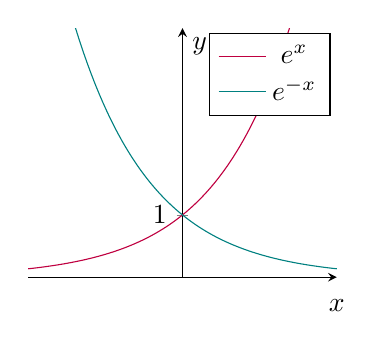
\begin{tikzpicture}
	\begin{axis}[
		axis lines = center,
		xlabel = \(x\),
		ylabel = {\(y\)},
		xmin=-2, xmax=2,
		ymin=0, ymax=4,
		xtick={0}, xticklabels={0},
		ytick={1}, yticklabels={1},
		x label style={at={(axis description cs:1,-0.05)},anchor=north},
	]
		\addplot [
			domain=-2:2,
			samples=100,
			color=purple,
			]
			{exp(x)};
		\addlegendentry{\(e ^{x}\)}
		\addplot [
			domain=-2:2,
			samples=100,
			color=teal,
			]
			{exp(-x)};
		\addlegendentry{\(e ^{-x}\)}
	\end{axis}
\end{tikzpicture}
\end{center}
\end{multicols}
\[
w(y_1,y_2)= \begin{vmatrix}
	e ^{x} & e ^{-x}\\ e ^{x} & -e ^{-x}
\end{vmatrix} = -1-1)-2\not=0
.\]
$\Rightarrow \{y_1;y_2\}$ is a fundamental system for the DE $y''-y=0$
\paragraph{Ex.:} $y''(x)-y'(x)=0,\quad y_1(x)=e ^{x},\quad y_2(x),\equiv 1$





\end{document}
